% =====================================================================
% INTERNSHIP NOTEBOOK - Todorut Aurel-Dan, group 30434
% Compile:  pdflatex internship_notebook.tex   (run it twice)
% Figures are expected in ./figures/
% =====================================================================
\documentclass[11pt,a4paper]{article}

\usepackage[utf8]{inputenc}
\usepackage[T1]{fontenc}
\usepackage[english]{babel}
\usepackage[margin=2.5cm]{geometry}
\usepackage{graphicx}
\usepackage{booktabs}
\usepackage{amsmath}
\usepackage{xcolor}
\usepackage{fancyhdr}
\usepackage{enumitem}
\usepackage[hidelinks]{hyperref}
\usepackage{caption}
\usepackage{float}              % gives [H] = put the float exactly here
\usepackage[section]{placeins}  % a float cannot drift into the next section

\graphicspath{{figures/}}
\captionsetup{font=small}
\setlist{itemsep=2pt, topsep=3pt}

\pagestyle{fancy}
\fancyhf{}
\fancyhead[L]{\small Internship Notebook}
\fancyhead[R]{\small Todoruț Aurel-Dan, group 30434}
\fancyfoot[C]{\small \thepage}

\title{\vspace{-1.5cm}\textbf{Internship Notebook}\\[0.3cm]
\large Deep Learning for Image Classification and Medical Image Segmentation}
\author{Todoruț Aurel-Dan}
\date{July -- August 2026}

\begin{document}
\maketitle
\thispagestyle{fancy}

% =====================================================================
\section{Header}
% =====================================================================

\begin{tabbing}
\hspace{6.4cm}\= \kill
\textbf{Group} \> 30434 \\[2pt]
\textbf{Student name and surname} \> Todoruț Aurel-Dan \\[2pt]
\textbf{Faculty} \> Faculty of Automation and Computer Science, \\
                 \> Technical University of Cluj-Napoca \\[2pt]
\textbf{Specialization} \> Computer Science, year 3 \\[2pt]
\textbf{Place of the internship} \> Faculty of Automation and Computer Science, \\
                 \> Str. George Barițiu no. 28, room 37, Cluj-Napoca \\[2pt]
\textbf{Internship period} \> 13.07.2026 -- 21.08.2026 (6 weeks) \\[2pt]
\textbf{Total number of hours} \> 200 hours \\[2pt]
\textbf{Tutor} \> Conf.dr.ing. Tiberiu Marita \\
                 \> tiberiu.marita@cs.utcluj.ro \\[2pt]
\textbf{Student contact} \> todorut.dan@yahoo.com
\end{tabbing}

% =====================================================================
\section{Summary}
% =====================================================================

During this internship I worked on 2 deep learning projects in PyTorch. The
first was image classification on CIFAR-10, where I built a convolutional neural
network from scratch and ran it on three tasks: cat versus dog (2 classes), only
the animal classes (6), and the full dataset (10). The best test accuracy was
88.25\% on the binary task and 88.85\% on the ten-class task. I also ran ten
experiments changing one setting at a time, to see which parts of the network
actually matter.

The second and larger project was medical image segmentation on the LiTS dataset
(Liver Tumor Segmentation). Here the goal is to give every pixel of a CT slice
one of three labels: background, liver or tumour. I implemented two
architectures, a standard U-Net and an Attention U-Net, and compared them under
identical conditions. The final foreground Dice scores were 0.8222 for U-Net and
0.8247 for Attention U-Net, so the attention gates did not give a real
improvement.

The first week was mostly learning, using the Stanford course material. After that I spent
about two weeks on classification and three weeks on segmentation.

What I did not expect is how much of the work is checking that results mean what
they seem to mean. I found that the first version of the segmentation dataset had
label files damaged by JPEG compression, that my first data split let almost
identical images appear in both training and test sets, and that pixel accuracy
looks good while the model finds nothing. Every one of those problems was
silent (no error message). I ended up writing small tools whose only job is to
verify my own work, and they caught several mistakes.

% =====================================================================
\section{Detailed description of the activities}
% =====================================================================

\subsection{Weekly diary}

% ---------------------------------------------------------------
\subsubsection*{Week 1 (13--17 July): setup and learning}

The first days went into preparing the environment and studying, because I had
only used neural networks in one course before and never on images of this size.

\textbf{Environment.} I installed Miniconda and made a separate conda
environment instead of installing packages into the system Python. It turned out to be very useful: later I broke a PyTorch
installation and, because everything was inside one environment, fixing it was a
matter of recreating that environment instead of repairing the whole system. I
installed PyTorch with CUDA support and checked that
\texttt{torch.cuda.is\_available()} returned \texttt{True}, so training would run
on my laptop GPU (NVIDIA RTX 3050) instead of the CPU. I used PyCharm as editor.

\textbf{Learning.} I went through the parts of Stanford (``Convolutional
Neural Networks for Visual Recognition'') that I needed, mainly the lectures on
convolution and pooling, on training neural networks, and the notes on
regularization. The ideas I had to understand before writing code were:

\begin{itemize}
  \item what a convolution filter computes, and why weight sharing lets one
        filter find the same pattern anywhere in the image;
  \item the receptive field, and why two stacked $3\times3$ convolutions see a
        $5\times5$ area but use fewer weights than one $5\times5$ filter;
  \item what max pooling does, and what information it throws away;
  \item batch normalization, dropout and data augmentation as three different
        ways of fighting overfitting.
\end{itemize}

I also read about segmentation, which was completely new to me. The main
change of thinking is that the output is not one label per image but one label
per pixel, so the network has to produce something the same size as its input.
That is where the (encoder -> decoder) shape comes from.


% ---------------------------------------------------------------
\subsubsection*{Week 2 (20--24 July): classification, implementation}

This week I built the classification project. I split the code into separate
files from the start, because I would want to run many experiments:
\texttt{config.py} (one object holding every setting), \texttt{data.py},
\texttt{model.py}, \texttt{train.py}, \texttt{evaluate.py} and
\texttt{gradcam.py}.

\textbf{Data.} CIFAR-10 has a train and a test split but no validation split, so
I cut a validation set out of the training data. This matters because if you tune
settings by looking at the test set, you are effectively training on it.
Augmentation was random horizontal flips and small random crops, applied only to
the training set and never to validation or test.

\textbf{Model.} The network is made of repeated blocks. Each block has one or
more $3\times3$ convolutions, each followed by batch normalization and ReLU, then
a max pooling layer that halves the resolution. The number of filters doubles
every block. After the last block a global average pooling layer flattens
everything, then one hidden fully connected layer, then the output layer with one
score per class. Everything is configurable, so I could change the depth or the
width from the command line without editing the model. The default network has
\textbf{320{,}994} trainable parameters.

\textbf{Three tasks from one codebase.} I made the set of classes a setting
instead of hard coding it, so the same code runs on cat versus dog, on the six
animal classes, and on all ten classes.

\begin{figure}[H]
\centering
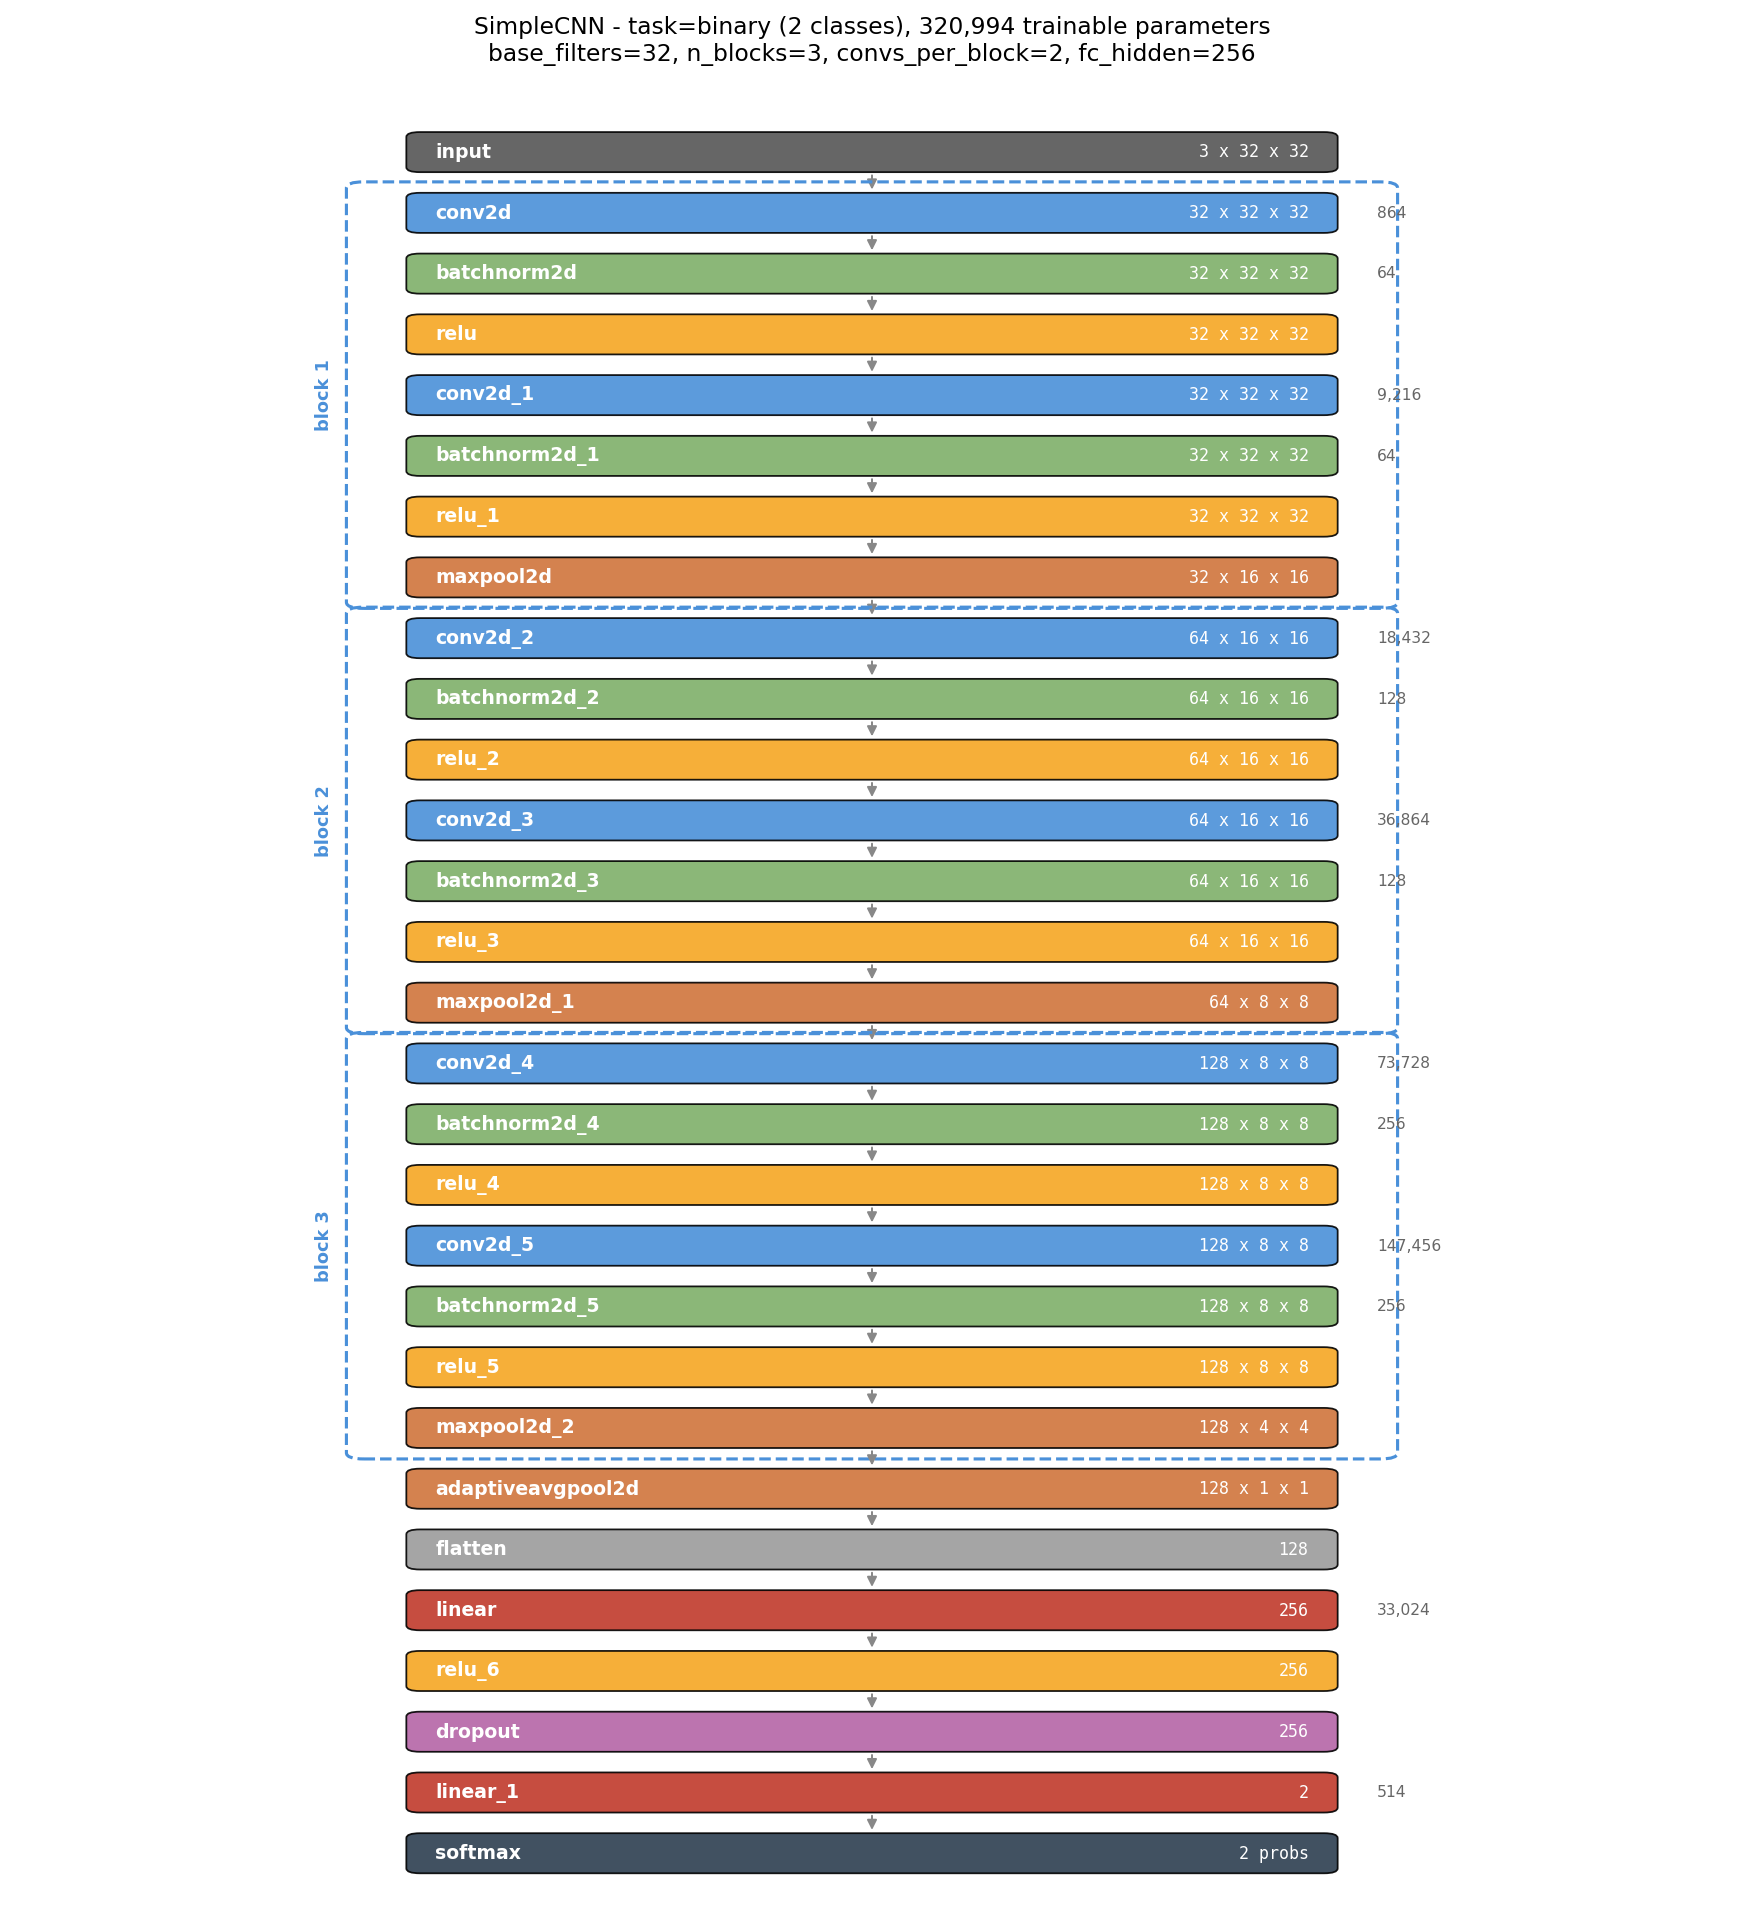
\includegraphics[width=0.62\textwidth]{cls_architecture.png}
\caption{The classification network for the binary task, drawn automatically from
the code. Three convolution blocks, each halving the resolution and doubling the
number of filters, then global average pooling and two fully connected layers.}
\end{figure}

\textbf{Problems.} Two things cost me time. On Windows the data loader crashed
with a memory error when I used several worker processes, each worker
imports PyTorch and Windows backs the shared memory with the paging file,
which was too small. I ran with zero workers instead. And my first runs were much
slower than they should have been until I realised the workers were being
recreated at every epoch.

% ---------------------------------------------------------------
\subsubsection*{Week 3 (27--31 July): classification experiments}

With the pipeline working, this week was about running experiments and
understanding results rather than writing new features.

\textbf{Metrics.} I implemented accuracy, balanced accuracy, macro F1, ROC-AUC
and a confusion matrix. The confusion matrix was the most useful, because it
shows which classes get mixed up and not only how often.

\textbf{Baselines.} Table~\ref{tab:cls_baselines} lists the three tasks.

\begin{table}[H]
\centering
\small
\begin{tabular}{lrrrrr}
\toprule
\textbf{Task} & \textbf{Classes} & \textbf{Epochs} & \textbf{Best val acc}
& \textbf{Test acc} & \textbf{Macro F1} \\
\midrule
Cat vs dog (binary) & 2  & 40 & 0.8850 & 0.8825 & 0.8825 \\
Animals only        & 6  & 50 & 0.8713 & 0.8680 & 0.8680 \\
Full CIFAR-10       & 10 & 50 & 0.8924 & 0.8885 & 0.8881 \\
\bottomrule
\end{tabular}
\caption{Baseline results for the three classification tasks.}
\label{tab:cls_baselines}
\end{table}

Something surprising here: the ten class task scores \emph{higher} than the
six class one, even though it has more classes. The reason is that CIFAR-10
contains four vehicle classes (airplane, automobile, ship, truck) which are easy
to separate from animals, while the six class task keeps only animals, which look
much more alike. More classes does not automatically mean a harder problem.

On the binary task the confusion matrix was $[[896, 104], [131, 869]]$: cat
recall 0.896, dog recall 0.869, so the errors were roughly balanced.

\begin{figure}[H]
\centering
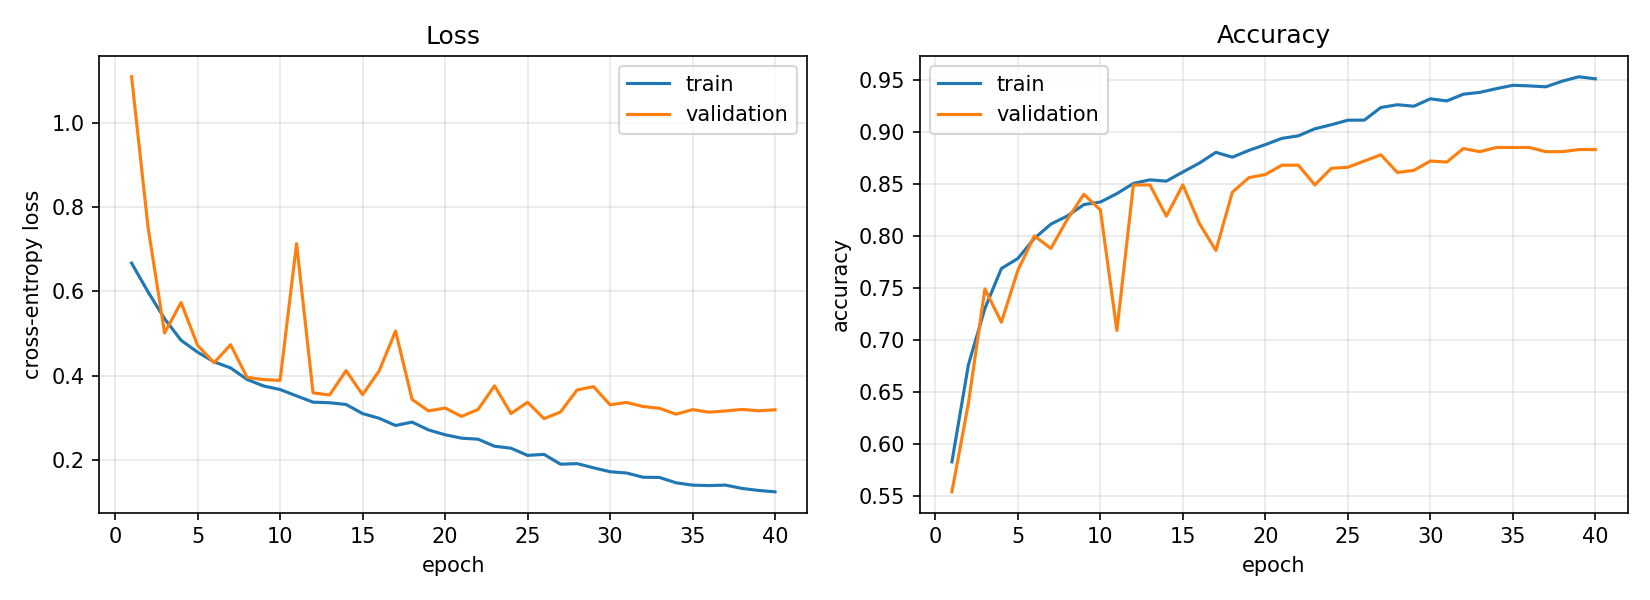
\includegraphics[width=0.58\textwidth]{cls_curves_binary.png}\hfill
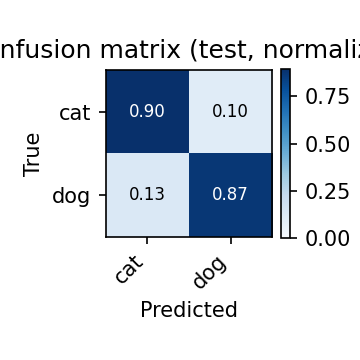
\includegraphics[width=0.38\textwidth]{cls_confusion_binary.png}
\caption{Binary task: training curves over 40 epochs (left) and the test
confusion matrix (right).}
\end{figure}

\textbf{Experiments.} I ran ten variants, each changing one thing, all for 20
epochs so they were comparable (Table~\ref{tab:cls_exp}). Because the budget is
shorter, the baseline here scores 0.8575 instead of the 0.8825 from the 40-epoch
run, the point of the table is the differences between rows, not the absolute
values.

\begin{table}[H]
\centering
\small
\begin{tabular}{llrrr}
\toprule
\textbf{Variant} & \textbf{What changed} & \textbf{Params}
& \textbf{Test acc} & \textbf{vs baseline} \\
\midrule
baseline         & 3 blocks, 32 filters, dropout 0.3, aug on & 320{,}994 & 0.8575 & -- \\
no\_dropout      & dropout 0 instead of 0.3        & 320{,}994   & \textbf{0.8720} & $+0.0145$ \\
wide\_64         & 64 base filters                 & 1{,}212{,}610 & 0.8695 & $+0.0120$ \\
deep\_4blocks    & 4 conv blocks instead of 3      & 1{,}239{,}522 & 0.8630 & $+0.0055$ \\
label\_smooth    & label smoothing 0.1             & 320{,}994   & 0.8580 & $+0.0005$ \\
convdrop         & spatial dropout 0.1 per block   & 320{,}994   & 0.8550 & $-0.0025$ \\
sgd              & SGD + momentum instead of Adam  & 320{,}994   & 0.8440 & $-0.0135$ \\
no\_augment      & no random crop or flip          & 320{,}994   & 0.8410 & $-0.0165$ \\
shallow\_2blocks & 2 conv blocks instead of 3      & 82{,}914    & 0.8130 & $-0.0445$ \\
no\_batchnorm    & BatchNorm removed               & 320{,}546   & \textbf{0.7735} & $\mathbf{-0.0840}$ \\
\bottomrule
\end{tabular}
\caption{Hyperparameter experiments on the binary task, 20 epochs each.}
\label{tab:cls_exp}
\end{table}

Three things I learned from this table:

\begin{itemize}
  \item \textbf{BatchNorm matters most by far.} Removing it costs 8.4 percentage
        points, more than every other change put together. It changes almost no
        parameters (320{,}546 versus 320{,}994), so this is not about capacity.
  \item \textbf{Dropout was actually hurting.} Turning it off improved
        test accuracy by 1.5 points. With augmentation already on, and a network
        this small, dropout was too much regularization.
  \item \textbf{Depth matters more than width.} Going from 3 blocks to 2 costs
        4.5 points while removing 74\% of the parameters, but going from 32 to
        64 filters buys only 1.2 points for four times the parameters.
\end{itemize}

\textbf{Overfitting test.} The experiment was a run designed to overfit:
no augmentation and no dropout. The gap between training and validation accuracy
grew to about 15 points and the validation loss started going up while
training loss kept falling. That is the picture of a model memorising
its training data.

\begin{figure}[H]
\centering
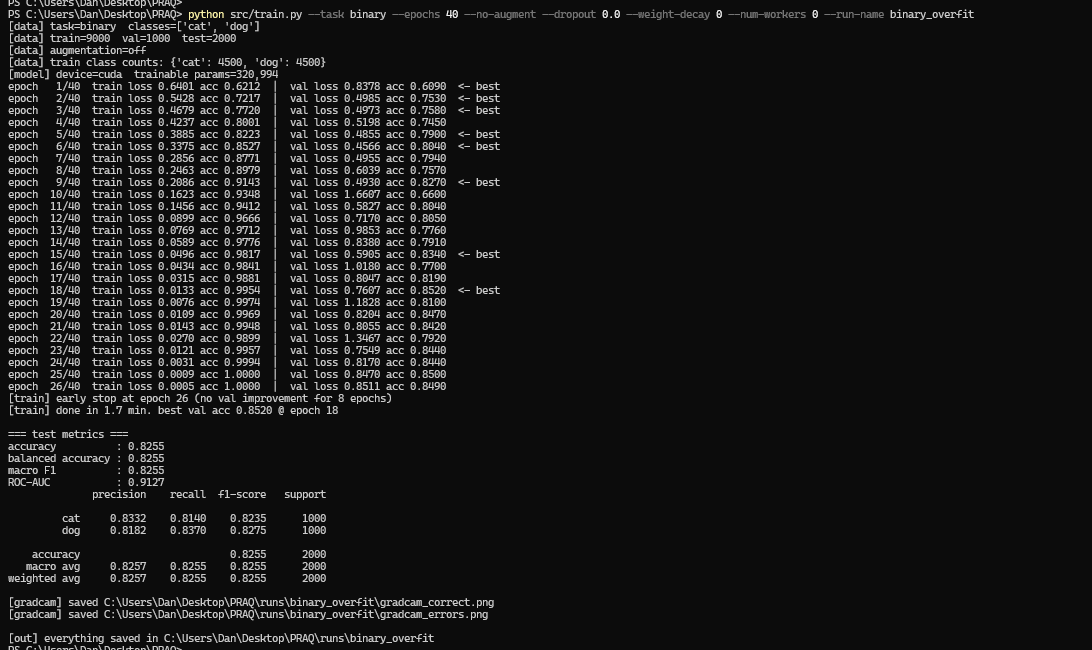
\includegraphics[width=0.72\textwidth]{cls_overfit.png}
\caption{The overfitting run: no augmentation and no dropout. Training accuracy
keeps climbing while validation accuracy stops improving, and the validation loss
turns upward. This is the signal to stop training or add regularization.}
\end{figure}

\textbf{Grad-CAM.} I implemented Grad-CAM to see which part of an image the
network was using. It takes the gradient of the predicted class with respect to
the last convolutional layer and turns it into a heat map over the input. I
produced one figure for correct predictions and one for mistakes. On the correct
ones the heat sits on the animal; on several mistakes it sits on the background,
which explains the error.

\begin{figure}[H]
\centering
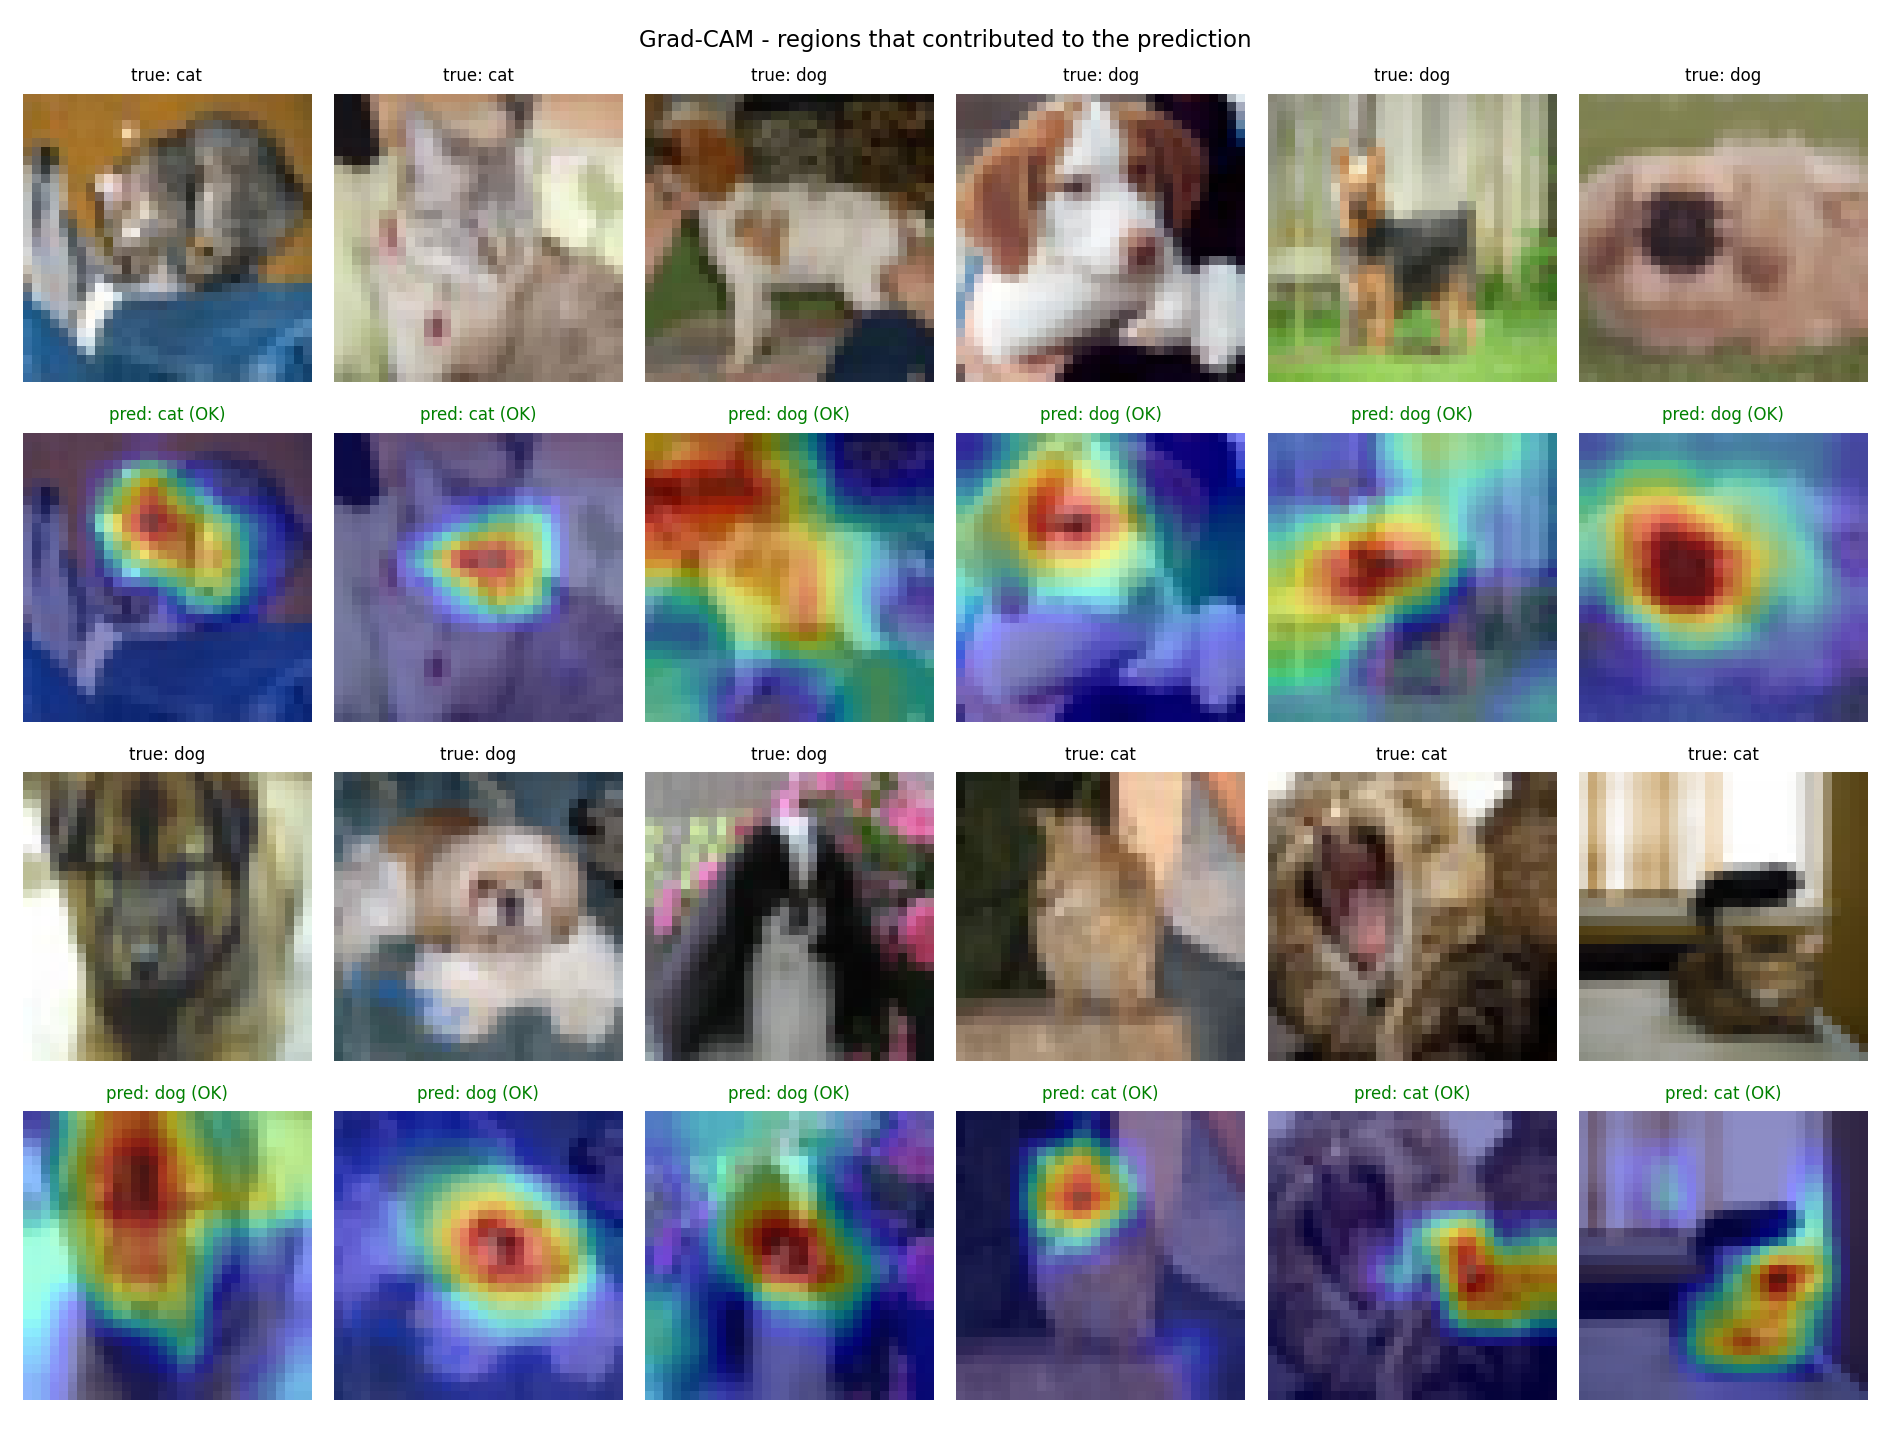
\includegraphics[width=0.48\textwidth]{cls_gradcam_correct.png}\hfill
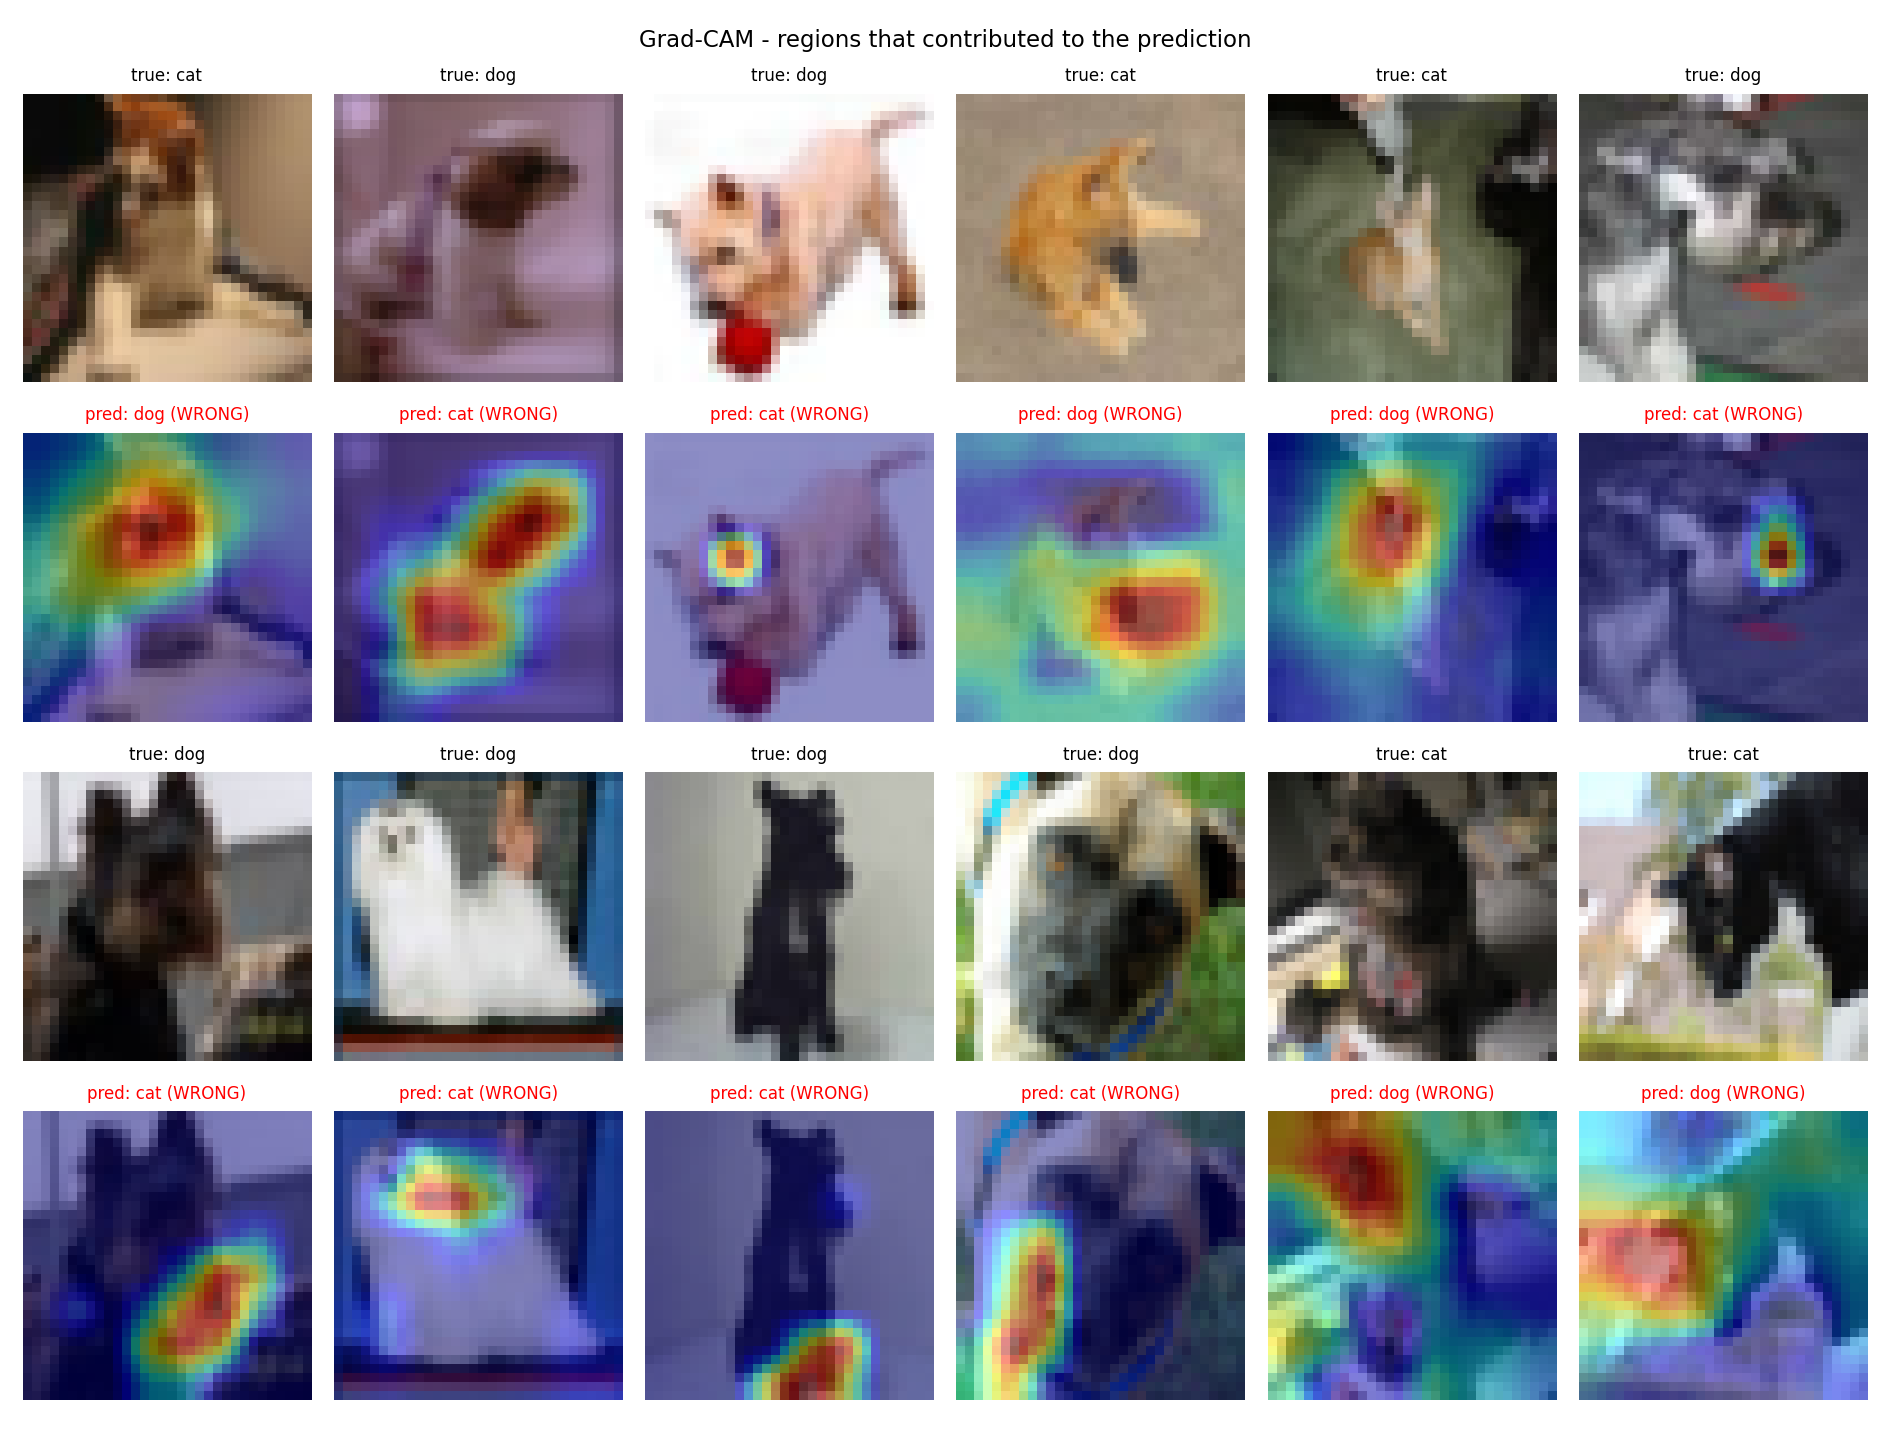
\includegraphics[width=0.48\textwidth]{cls_gradcam_errors.png}
\caption{Grad-CAM on correct predictions (left) and on mistakes (right).}
\end{figure}


% ---------------------------------------------------------------
\subsubsection*{Week 4 (3--7 August): segmentation, learning and dataset study}

The second project was segmentation of the liver and liver tumours in CT slices.
This was harder in every way, so the first part of the week was reading again.

\textbf{Learning.} I studied the U-Net architecture and skip connections, then
the Attention U-Net idea of filtering those skip connections with attention
gates. I also had to learn some CT basics: what an axial slice is, what
Hounsfield Units are, and why the liver only appears in part of a scan.

\textbf{Dataset study.} Instead of coding immediately, I wrote a program that
only reads the dataset and describes it. This was the best decision of the whole
internship, because it found real problems:

\begin{itemize}
  \item \textbf{131 patients}, \textbf{58{,}638} slices of $256\times256$ pixels,
        with between 74 and 987 slices per patient.
  \item \textbf{67.4\% of slices contain no liver at all}, because a scan covers
        more of the body than the liver. Training on them mostly teaches the
        network to answer ``background''.
  \item The classes are extremely unbalanced: background 97.74\%, liver 2.15\%,
        tumour \textbf{0.12\%}. Background is about 840 times more common than
        tumour.
  \item The first version of the dataset I downloaded stored the masks as
        \textbf{JPEG}. JPEG is lossy, which is fine for photographs but wrong for
        label images, where the pixel value \emph{is} the class number. I found
        pixels with value 3 in a dataset that only has classes 0, 1 and 2, which
        proves the labels had been changed by compression.
\end{itemize}

Because of that last point I switched to a \textbf{PNG} version of the same
dataset, which is lossless. In that version the two label classes are stored as
two separate binary masks per slice, one for the liver and one for the lesion,
which have to be merged into a single three class mask. The merge order matters:
the liver mask also covers the lesion, so the lesion must be written last.
Otherwise every tumour pixel is overwritten and the class disappears completely,
with no error message.

% ---------------------------------------------------------------
\subsubsection*{Week 5 (10--14 August): segmentation implementation}

\textbf{Data pipeline.} The important detail is how the data is split. My first
version split slices randomly, which is wrong: slices 240 and 241 of the same
patient are a few millimetres apart and look almost identical, so a random split
puts nearly the same image in both training and test. The scores look good but
they measure memorisation. I changed it to split \textbf{whole patients}: the 131
patients are shuffled and divided, and every slice follows its patient. The
scores dropped and became honest. The final split is 91 / 20 / 20 patients,
giving 13{,}745 / 3{,}151 / 2{,}247 slices.

Augmentation needed care too. The image and its mask must get exactly the
same random transformation, or the labels stop matching the picture. I used only
flips and 90-degree rotations, because those keep mask values as exact integers,
and masks are always resized with nearest neighbour interpolation, never
bilinear, interpolating between class 1 and class 2 would invent a class 1.5.

\textbf{Models.} I built both architectures from the same blocks so the
comparison would be fair: \texttt{DoubleConv} (two $3\times3$ convolutions with
batch normalization and ReLU), \texttt{Down} (max pooling then
\texttt{DoubleConv}), \texttt{Up} (transposed convolution, concatenate the skip,
then \texttt{DoubleConv}) and \texttt{AttentionGate}, used only in the Attention
U-Net.

\textbf{Loss.} Because of the imbalance I used Dice loss combined with
cross-entropy. Dice is computed per class and divided by that class's own size,
so tumour counts as much as background even though it is 840 times smaller. Plain
cross-entropy on its own would be dominated by background.

\textbf{Metrics.} I computed a confusion matrix and then Dice, IoU, precision and
recall per class. I did not use pixel accuracy as the main number: a
model predicting ``background'' everywhere scores about 97\% accuracy and
segments nothing. The number I used to pick the best model is the \textbf{mean
foreground Dice}, averaging only liver and tumour.


% ---------------------------------------------------------------
\subsubsection*{Week 6 (17--21 August): training, comparison, documentation}

\textbf{First runs.} I trained on my laptop GPU first. One epoch took about 6
minutes, so 40 epochs took just under 4 hours. While it ran I watched
\texttt{nvidia-smi} and saw GPU utilisation of only about 68\% with temperature
at 84--86\,\textdegree C, meaning the GPU was partly waiting for data and also
thermally limited.

\textbf{A better GPU.} Workstation with an RTX 2070,
which I used over remote desktop. I set up the same conda environment there,
copied the code, and downloaded the dataset again locally instead of transferring
3.4~GB over the remote connection. On Linux the data loader could use several
worker processes -- the thing that crashed on Windows, and utilisation went to
\textbf{98\%} with temperature down to 66\,\textdegree C. I ran training inside
\texttt{tmux} so the job would survive the remote connection dropping, which it
did more than once.


\textbf{Documentation.} Finally I generated the architecture diagrams and
parameter tables automatically from the code, so they cannot go out of date, and
wrote a tool that produces the comparison table and figures.

% ---------------------------------------------------------------
\subsection{Project description: liver and tumour segmentation}

This section describes the larger project in detail. My personal contribution is
the whole implementation, data pipeline, both architectures, loss, metrics,
training loop, evaluation and checking tools. I did not use an existing
segmentation framework.

\subsubsection*{Problem}

Given one axial CT slice of the abdomen, label every pixel as background, liver
or tumour. The motivation is that radiologists currently outline the liver and
every lesion by hand across hundreds of slices per patient, which is slow and
differs between readers.

\subsubsection*{Dataset}

LiTS (Liver Tumor Segmentation Benchmark), the version exported as 2D PNG slices.
Table~\ref{tab:data} lists the properties that changed my design.

\begin{table}[H]
\centering
\small
\begin{tabular}{lll}
\toprule
\textbf{Property} & \textbf{Value} & \textbf{What it forced} \\
\midrule
Patients & 131 & split by patient, not by slice \\
Slices & 58{,}638 at $256\times256$ & \\
Slices with no liver & 67.4\% & dropped from training \\
Usable slices & 19{,}143 & \\
Background pixels & 97.74\% & accuracy is meaningless \\
Liver pixels & 2.15\% & \\
Tumour pixels & 0.12\% & Dice based loss needed \\
Masks & 2 binary PNGs per slice & merged, lesion written last \\
\bottomrule
\end{tabular}
\caption{Dataset properties and the design decision each one forced.}
\label{tab:data}
\end{table}

\subsubsection*{Architectures}

Both networks share the same encoder and decoder. The encoder halves the
resolution four times while doubling the channels
($32 \rightarrow 64 \rightarrow 128 \rightarrow 256 \rightarrow 512$), so a
$256\times256$ input becomes $16\times16$ at the bottleneck. The decoder does the
reverse, and at every level it concatenates a skip connection carrying the
high resolution detail that pooling threw away.

The only difference is what happens to those skips:

\begin{itemize}
  \item \textbf{U-Net}: the skip is concatenated exactly as the encoder produced
        it, so everything crosses over, kidneys, spine, bowel and all.
  \item \textbf{Attention U-Net}: the skip first goes through an attention gate.
        The gate takes the coarser tensor from the level below as a ``gating
        signal'', combines it with the skip using $1\times1$ convolutions, and
        produces a weight $\alpha \in (0,1)$ per pixel. The skip is multiplied by
        $\alpha$ before being concatenated, so regions the decoder thinks are
        irrelevant get suppressed:
\end{itemize}
\[
\alpha = \sigma\!\left(\psi\!\left(\mathrm{ReLU}\!\left(W_g\,g + W_x\,x\right)\right)\right),
\qquad \text{output} = x \odot \alpha .
\]

The parameter counts are \textbf{7{,}762{,}531} for U-Net and
\textbf{7{,}894{,}783} for Attention U-Net. The difference,
\textbf{132{,}252 parameters (1.7\%)}, is exactly the four attention gates. That
makes this a clean comparison, because nothing else changes.

\begin{figure}[p]
\centering
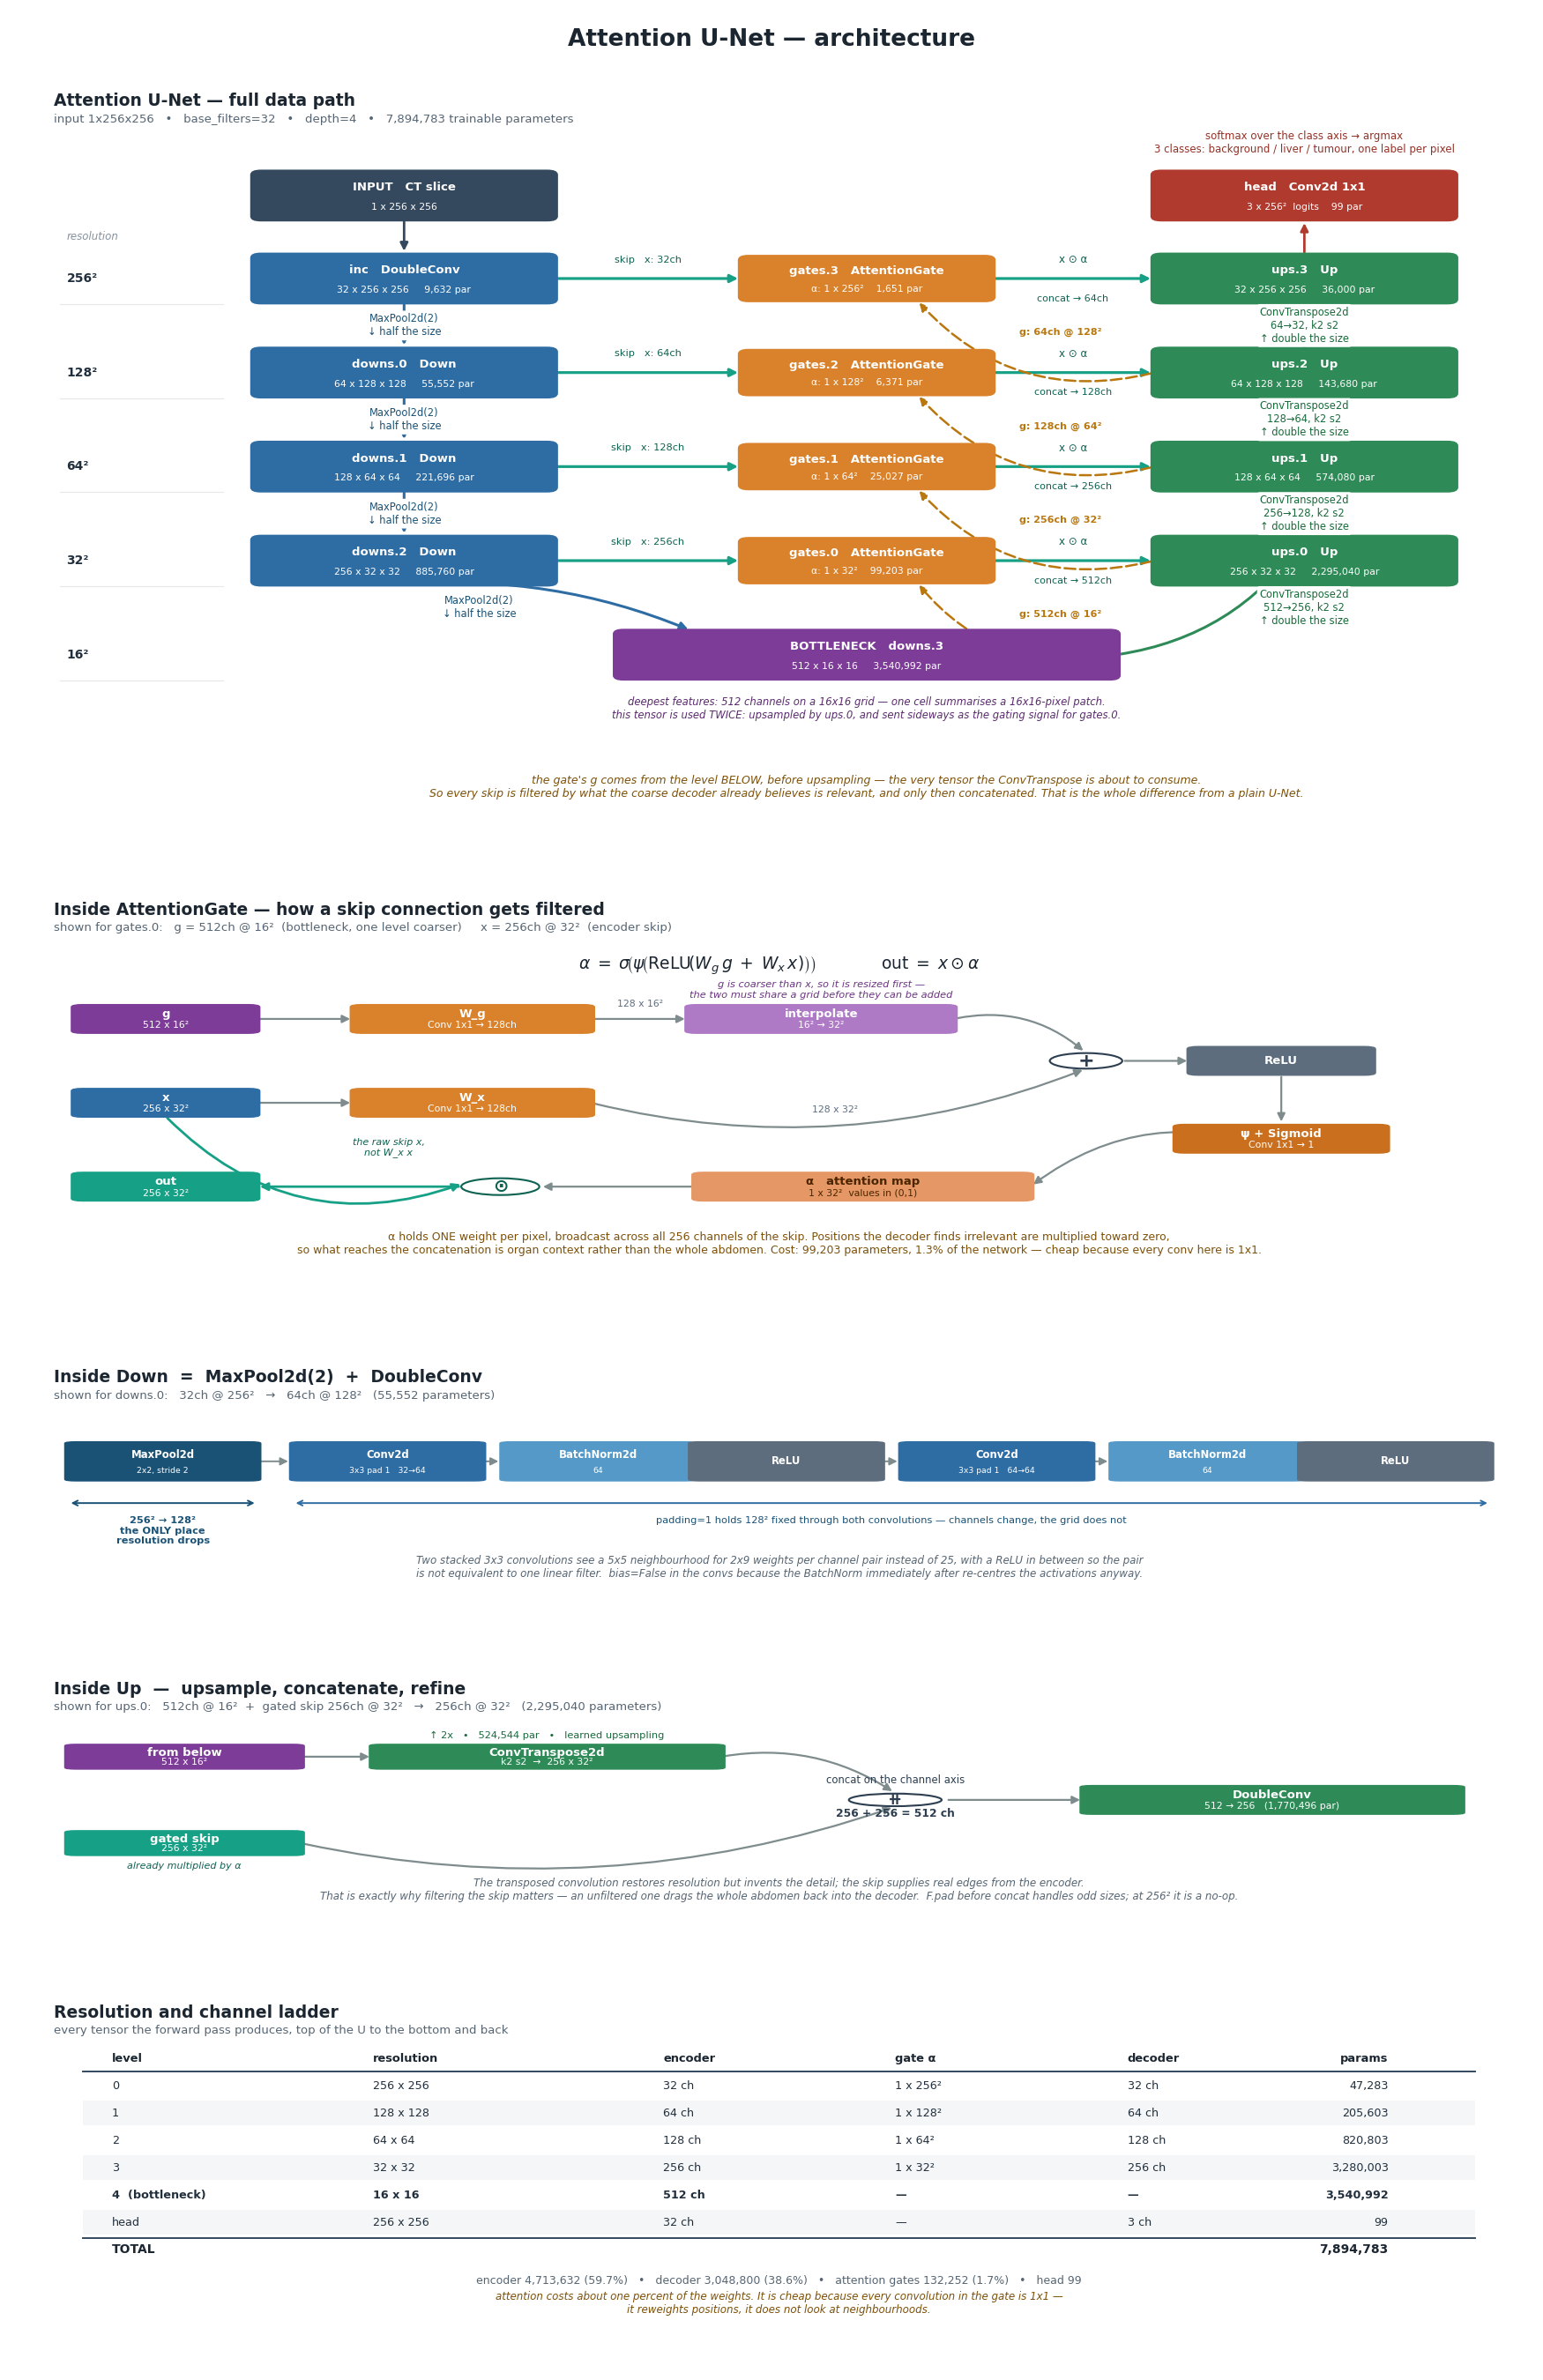
\includegraphics[height=0.86\textheight,keepaspectratio]{attention_unet_diagram.png}
\caption{Attention U-Net, generated automatically from the code so the shapes and
parameter counts cannot drift from the implementation. The orange boxes are the
four attention gates sitting on the skip connections; the dashed arrows are the
gating signals coming from the level below.}
\end{figure}


\subsubsection*{Training setup}

Dice + cross-entropy loss; Adam with learning rate $10^{-3}$ and weight decay
$10^{-4}$; cosine annealing over 40 epochs; batch size 8; mixed precision;
augmentation by flips and 90\textdegree{} rotations with identical parameters for
image and mask; model chosen by highest mean foreground Dice on validation; the
same seed (42) for both runs so both see the same split.

\subsubsection*{Results}

\begin{table}[H]
\centering
\small
\begin{tabular}{lrrrrr}
\toprule
\textbf{Model} & \textbf{Parameters} & \textbf{fg Dice} & \textbf{Liver Dice}
& \textbf{Tumour Dice} & \textbf{Time} \\
\midrule
U-Net (baseline) & 7{,}762{,}531 & 0.8222 & 0.9101 & \textbf{0.7343} & 93 min \\
Attention U-Net  & 7{,}894{,}783 & \textbf{0.8247} & \textbf{0.9172} & 0.7322 & 112 min \\
\bottomrule
\end{tabular}
\caption{Final test results. Both models trained 40 epochs on the same split with
the same seed.}
\label{tab:results}
\end{table}

\begin{figure}[H]
\centering
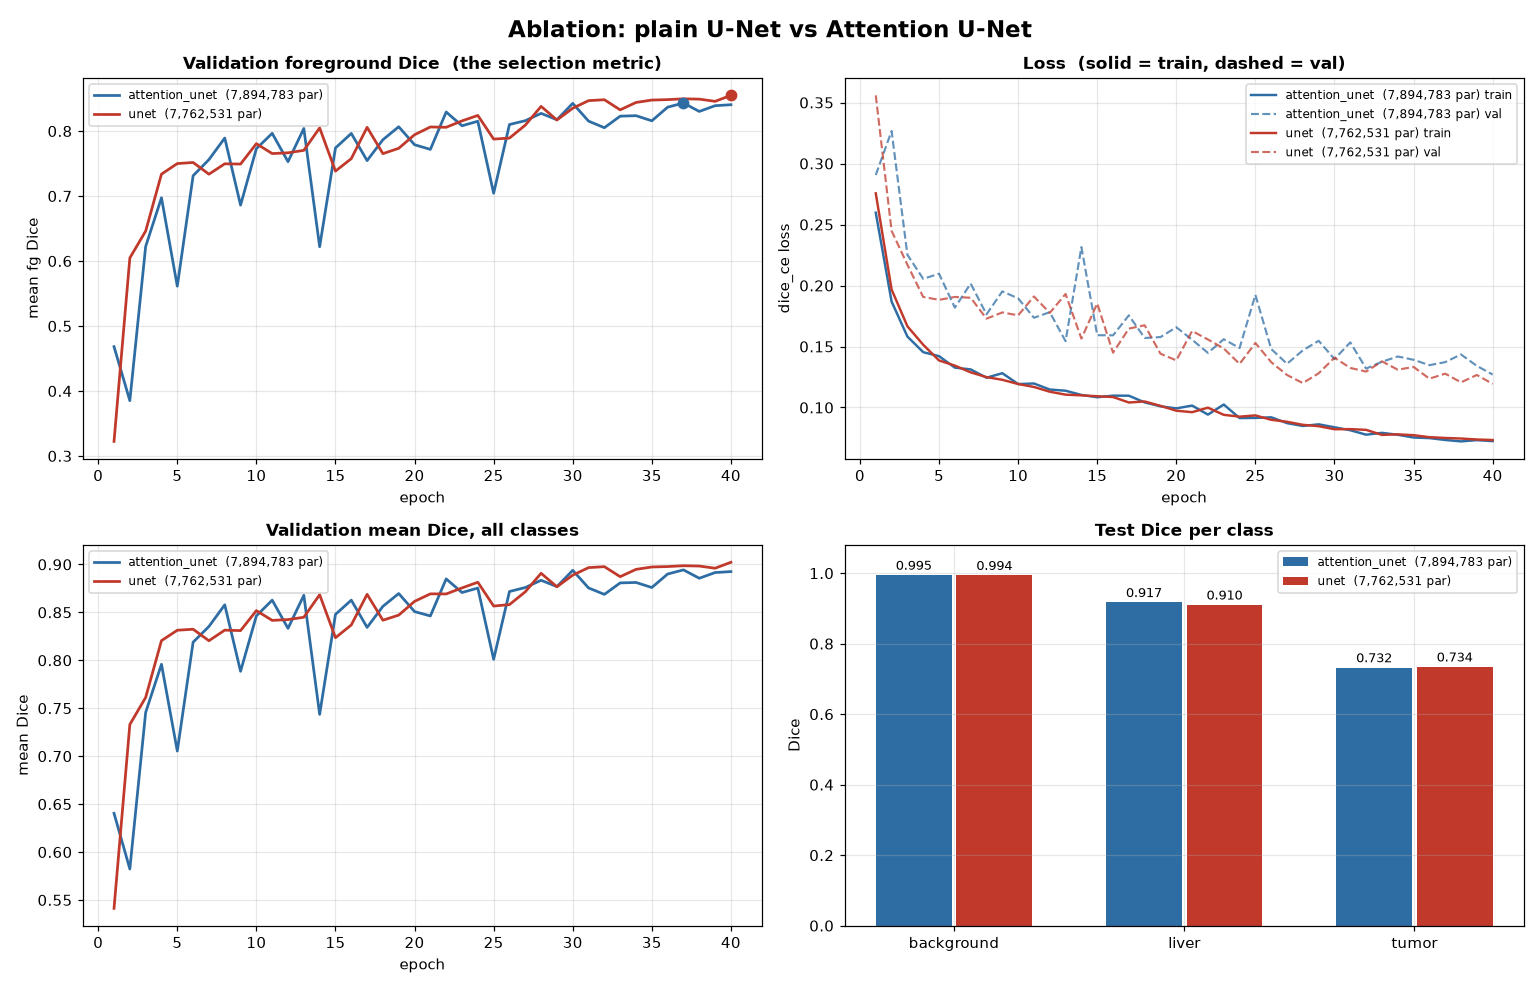
\includegraphics[width=\textwidth]{comparison_ablation.png}
\caption{Comparison of the two models. Top left is the metric used to select the
best epoch. The loss curves lie almost on top of each other and the per-class
bars show how small the differences are.}
\end{figure}

\textbf{The difference is not meaningful.} Attention U-Net is 0.0025 higher on
foreground Dice and 0.0071 higher on liver, but 0.0021 \emph{lower} on tumour.
The differences point in different directions depending on the metric, which is
what noise looks like. With one run per architecture, anything below about 0.02
cannot be separated from run-to-run variation. Attention U-Net also took 20\%
longer to train.

\textbf{Where the real difficulty is.} The interesting numbers are not the
comparison but the tumour class. For Attention U-Net, tumour precision is 0.816
but recall is only \textbf{0.664}, so when it says tumour it is usually right,
but it \textbf{misses a third of the actual disease}. Of the 582 test slices
containing a real lesion, \textbf{154 (26\%)} scored a Dice of exactly zero,
meaning the lesion was missed completely. The model is cautious, which for a
screening tool is the wrong direction -- you would rather over-flag and let a
radiologist dismiss it.

\textbf{Why accuracy would have hidden all of this.} A model predicting
background everywhere scores 93.4\% pixel accuracy on this test set. My trained
model scores 98.9\%. That looks like a small gain, but the foreground Dice went
from 0.000 to 0.825. Same two models, two metrics, completely different stories.

\begin{figure}[H]
\centering
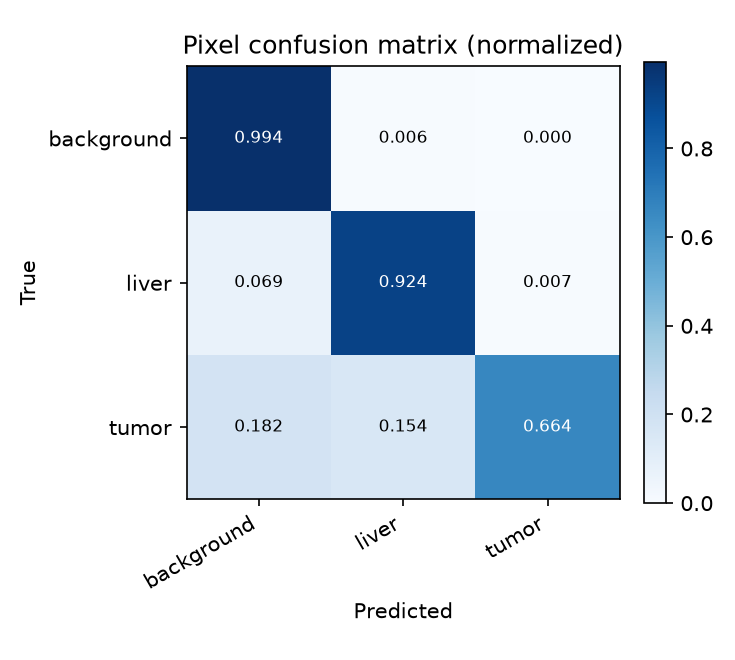
\includegraphics[width=0.55\textwidth]{attention_unet_confusion_test.png}
\caption{Normalized confusion matrix, Attention U-Net. Rows are the true class.
The tumour row is the important one: 66.4\% correct, 15.4\% predicted as liver,
and 18.2\% predicted as background -- which means the model missed the liver at
that location entirely.}
\end{figure}

\begin{figure}[H]
\centering
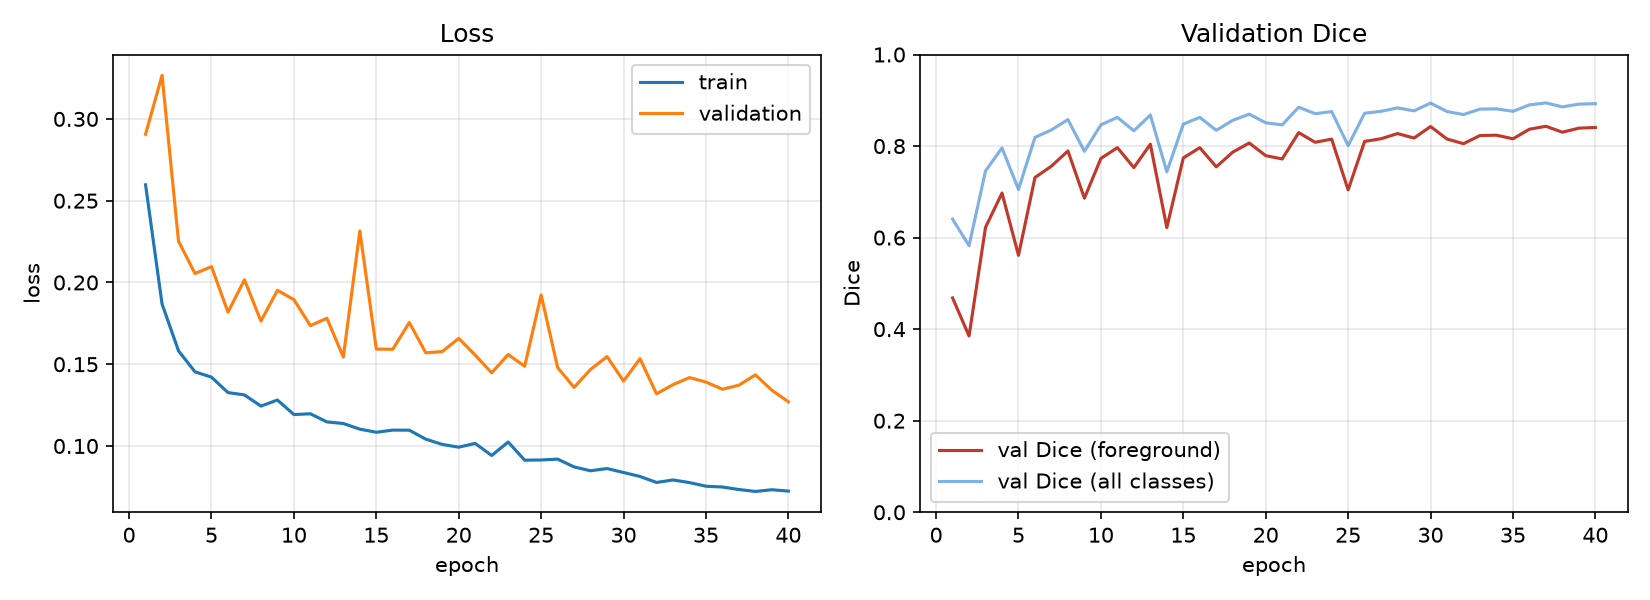
\includegraphics[width=0.85\textwidth]{attention_unet_training_curves.png}
\caption{Training curves. Training loss keeps falling while validation loss
flattens after about epoch 20, which is mild overfitting. Validation foreground
Dice (red, right) is the metric used to choose the best epoch.}
\end{figure}

\begin{figure}[p]
\centering
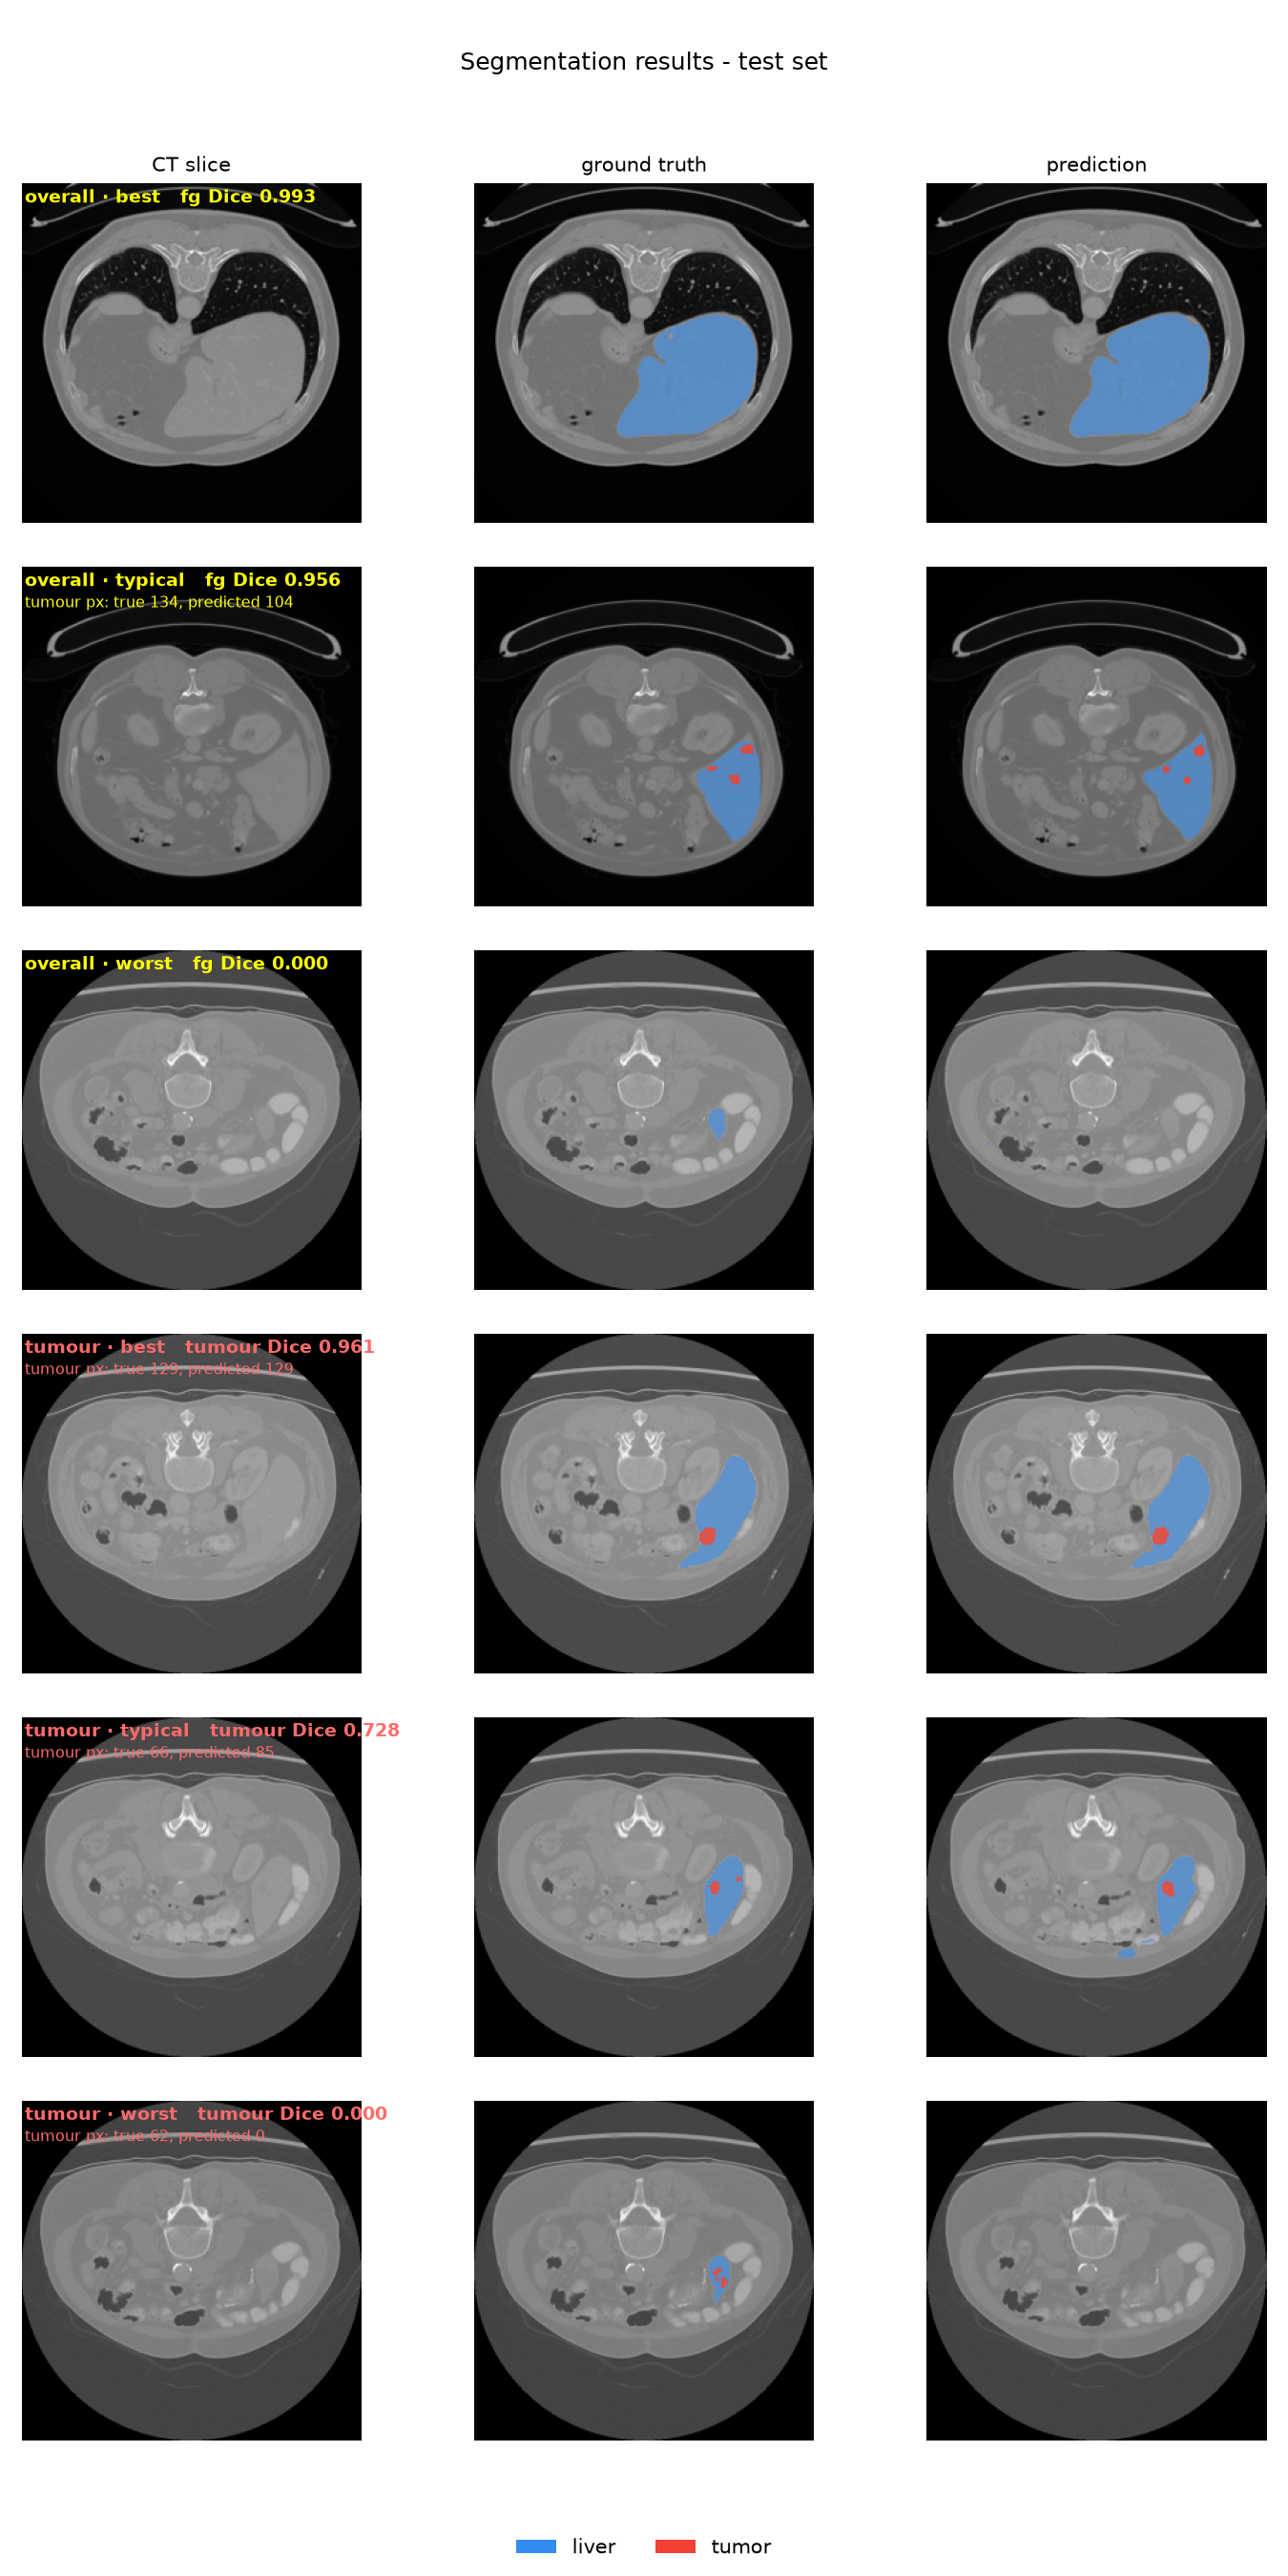
\includegraphics[height=0.86\textheight,keepaspectratio]{attention_unet_predictions_test.png}
\caption{Test predictions, Attention U-Net. Each row shows the CT slice, the
ground truth drawn by a radiologist, and the model output. The rows are chosen as
best, typical and worst by Dice, and the last rows are picked from slices that
contain a real lesion, so the figure shows the failures as well as the successes.}
\end{figure}

\textbf{Did the attention gates learn anything?} Since the numbers showed no
improvement, I extracted the $\alpha$ maps from the trained model to check
whether the gates were doing anything at all. They were: $\alpha$ was clearly
higher inside the liver than outside it, and the maps follow the shape of the
organ, getting sharper at higher resolution. So the mechanism works, it just does
not help on this task. My explanation is that the liver is large, has good
contrast and is always in roughly the same place, so the decoder does not need
help finding it -- and dropping the 67\% of empty slices already solves part of
the same problem.

\subsubsection*{Personal contributions}

\begin{itemize}
  \item Wrote the whole codebase with no segmentation framework: configuration,
        data pipeline, both architectures, loss, metrics, training loop,
        evaluation and figures.
  \item Found that the first dataset version had labels damaged by JPEG
        compression, and moved to a lossless PNG version.
  \item Found and fixed a data leakage problem by changing from a slice level to
        a patient level split.
  \item Chose foreground Dice instead of accuracy or loss for model selection,
        and showed with a concrete number why accuracy is misleading here.
  \item Wrote a self test tool and a dataset checking tool that caught several
        silent bugs, including an incomplete dataset download.
  \item Generated the architecture documentation automatically from the code, with
        a check that the diagram, the layer table and the model all agree on the
        parameter count.
\end{itemize}

\subsubsection*{Limitations}

\begin{itemize}
  \item Only one training run per architecture, so the comparison is not
        statistically significant.
  \item Dice is pooled over all test pixels, not averaged per patient. The LiTS
        benchmark reports per patient scores, so my numbers are not directly
        comparable to published results.
  \item The 2D 8-bit export destroys the Hounsfield Unit scale that real
        volumetric methods use, which limits how good any model on this data can
        be.
  \item Mean image brightness varies between patients from 95 to 182, and I use
        one fixed normalisation for all of them. Per image normalisation would
        probably help and is the first thing I would try next.
\end{itemize}

% =====================================================================
\section{Conclusions}
% =====================================================================

The most valuable thing I learned was not how to write a neural network. That
part is well documented and the code is fairly short. What surprised me is how
much of the work is making sure the numbers mean what you think they mean. Almost
every real problem I hit was silent: a dataset with corrupted labels that still
loaded fine, a data split that gave good scores for the wrong reason, a metric
that looked excellent while the model segmented nothing, a comparison ruined by
unequal training budgets, and a half downloaded dataset that produced plausible
but wrong results. None of these caused an error message. I only found them
because I checked.

That changed how I work. By the end I was writing a small verification tool
alongside each feature, and it saved more time than it cost. Computing the same
quantity two different ways and comparing them caught real mistakes.

Technically, I now understand convolutional networks, encoder decoder
architectures and attention mechanisms well enough to implement them. I also got practical experience I did not
have before: setting up CUDA environments on Windows and on Linux, using tmux, and reading GPU telemetry to discover that my
bottleneck was data loading rather than computation.

The negative parts were mostly environment problems rather than the work itself.
I lost most of a day to a PyTorch installation that broke in a way that looked
like a bug in my own code, and the Windows paging file limit blocked features
that worked immediately on Linux.

This internship made me more interested in medical image analysis and in
computer vision in general. What I find appealing is that the problems are not
only about architecture: the data is difficult and imperfect, the metrics need
thought, and being wrong has real consequences.

\end{document}
